\documentclass{beamer}
\usepackage{graphicx}
\usepackage{amsmath}

\title{Detailed Explanations of Macroeconomic Concepts}
\author{Charles Ancel}
\date{July 3, 2024}

\begin{document}

\frame{\titlepage}

\section{Relationship Between Real and Nominal Interest Rates and Their Effect on Consumption}
\begin{frame}
    \frametitle{Real and Nominal Interest Rates}
    \begin{itemize}
        \item \textbf{Nominal Interest Rate:} The stated interest rate on a loan or investment, not adjusted for inflation.
        \item \textbf{Real Interest Rate:} Adjusts the nominal rate to remove the effects of inflation.
        \begin{equation*}
            \text{Real Interest Rate} = \text{Nominal Interest Rate} - \text{Inflation Rate}
        \end{equation*}
    \end{itemize}
\end{frame}

\begin{frame}
    \frametitle{Effect on Consumption}
    \begin{itemize}
        \item \textbf{Low Real Interest Rates:}
        \begin{itemize}
            \item Borrowing is cheaper, encouraging loans for consumption and investment.
            \item Increases overall consumer spending.
        \end{itemize}
        \item \textbf{High Real Interest Rates:}
        \begin{itemize}
            \item Borrowing is more expensive, discouraging loans.
            \item Increases savings, reducing current spending.
        \end{itemize}
    \end{itemize}
\end{frame}

\begin{frame}
    \frametitle{Graph: Real and Nominal Interest Rates}
    \begin{center}
        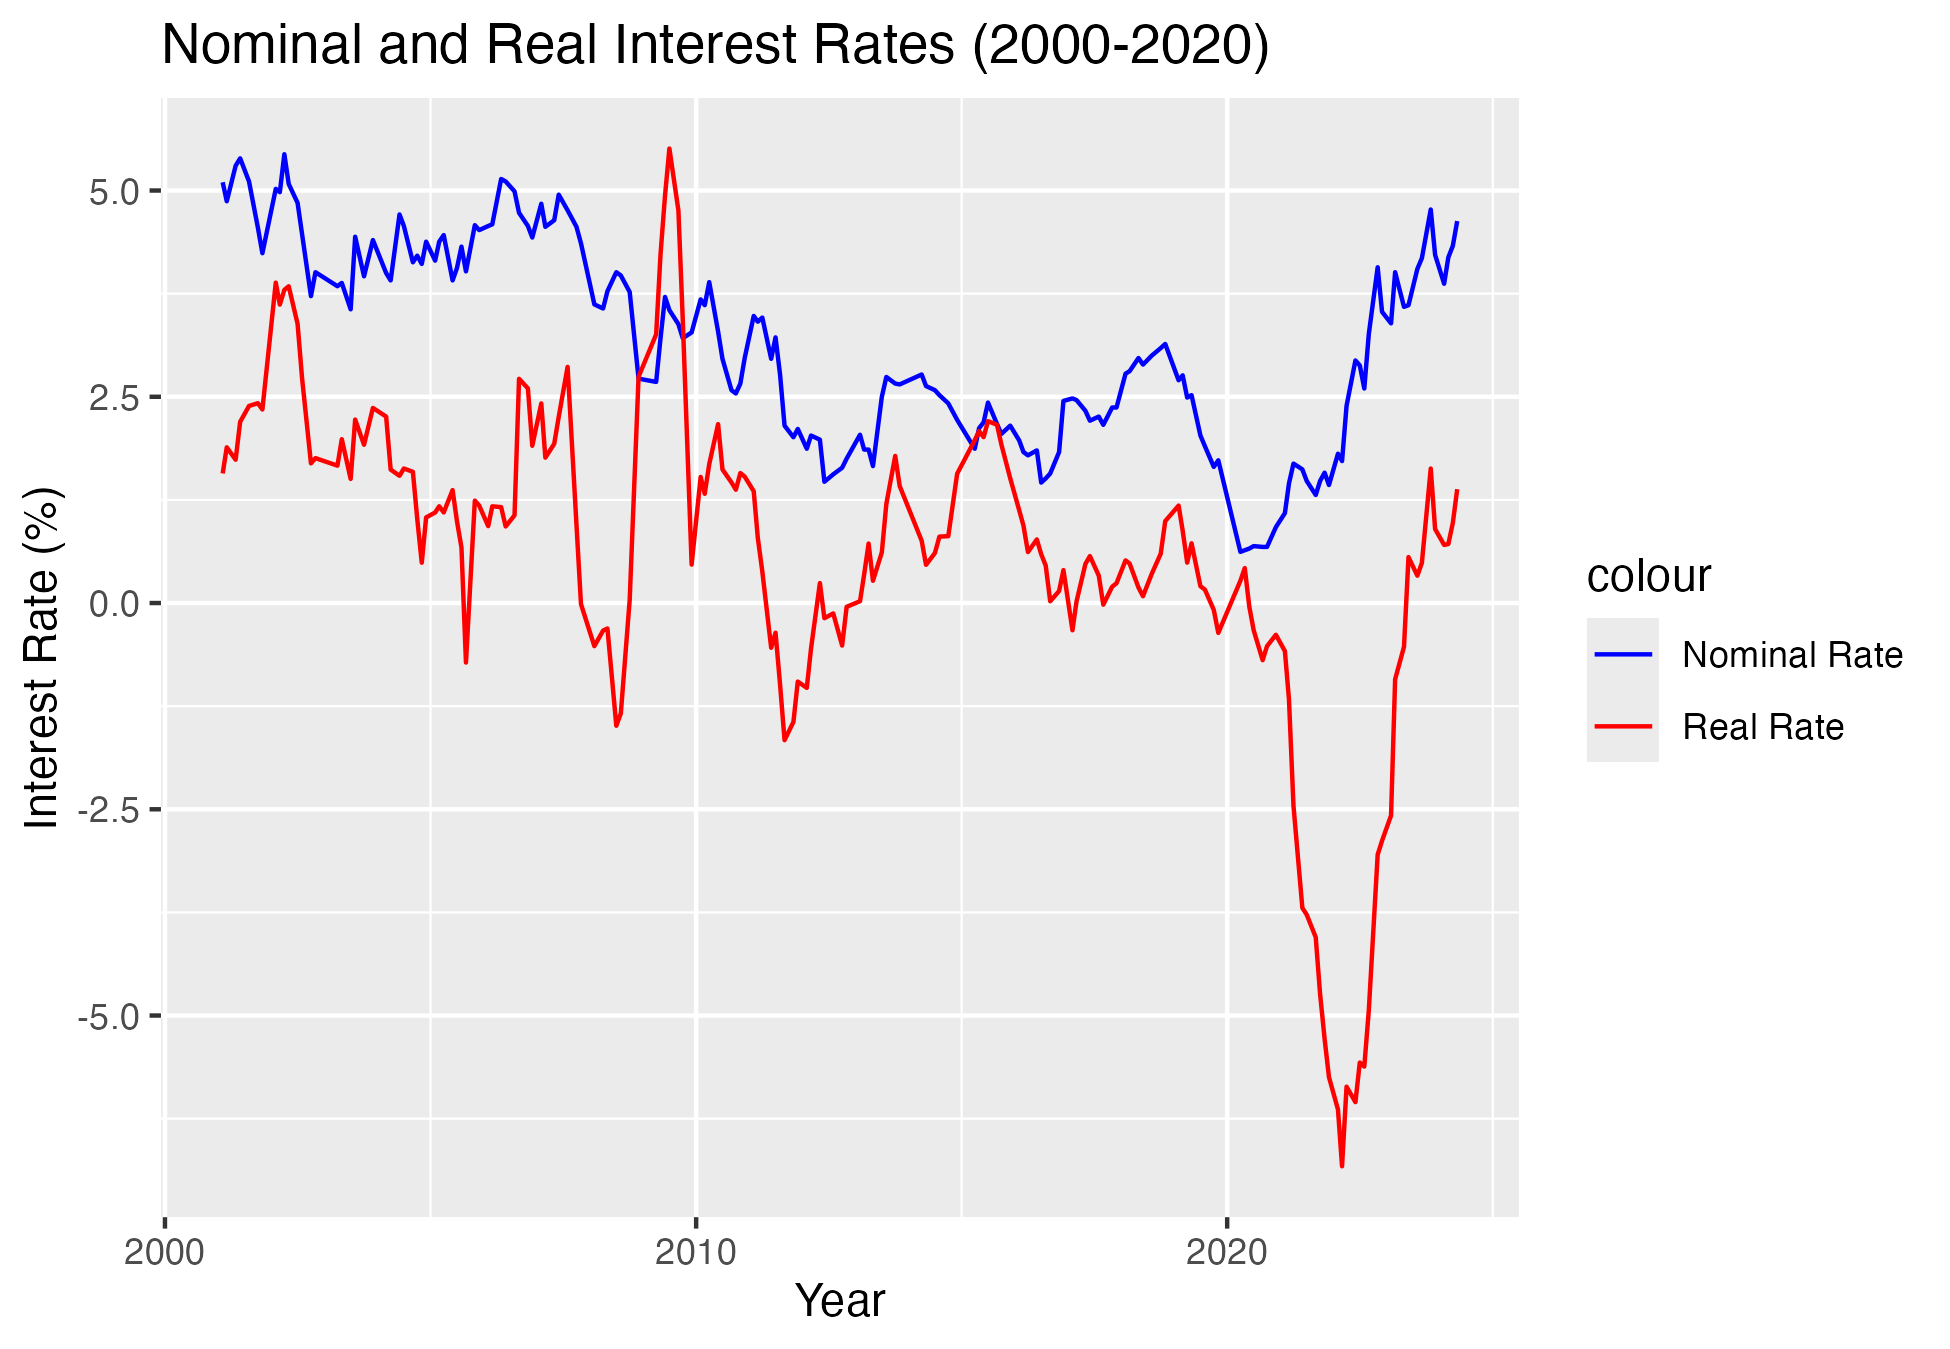
\includegraphics[width=0.9\textwidth]{/Users/cancel/Personal/Coursework/Econ425/VA1/R/Nominal_vs_Real_Interest_Rates.png}
    \end{center}
\end{frame}

\section{Debt Constraints and Policy Decisions}
\begin{frame}
    \frametitle{Debt Constraints}
    \begin{itemize}
        \item \textbf{Debt Constraints:} Limitations on consumers' ability to borrow money.
        \item \textbf{Assuming No Debt Constraints:}
        \begin{itemize}
            \item Policies may overestimate the impact of fiscal or monetary measures.
            \item Can lead to ineffective policy measures, increased inequality, and economic instability.
        \end{itemize}
    \end{itemize}
\end{frame}

\begin{frame}
    \frametitle{Graph: Total Consumer Credit}
    \begin{center}
        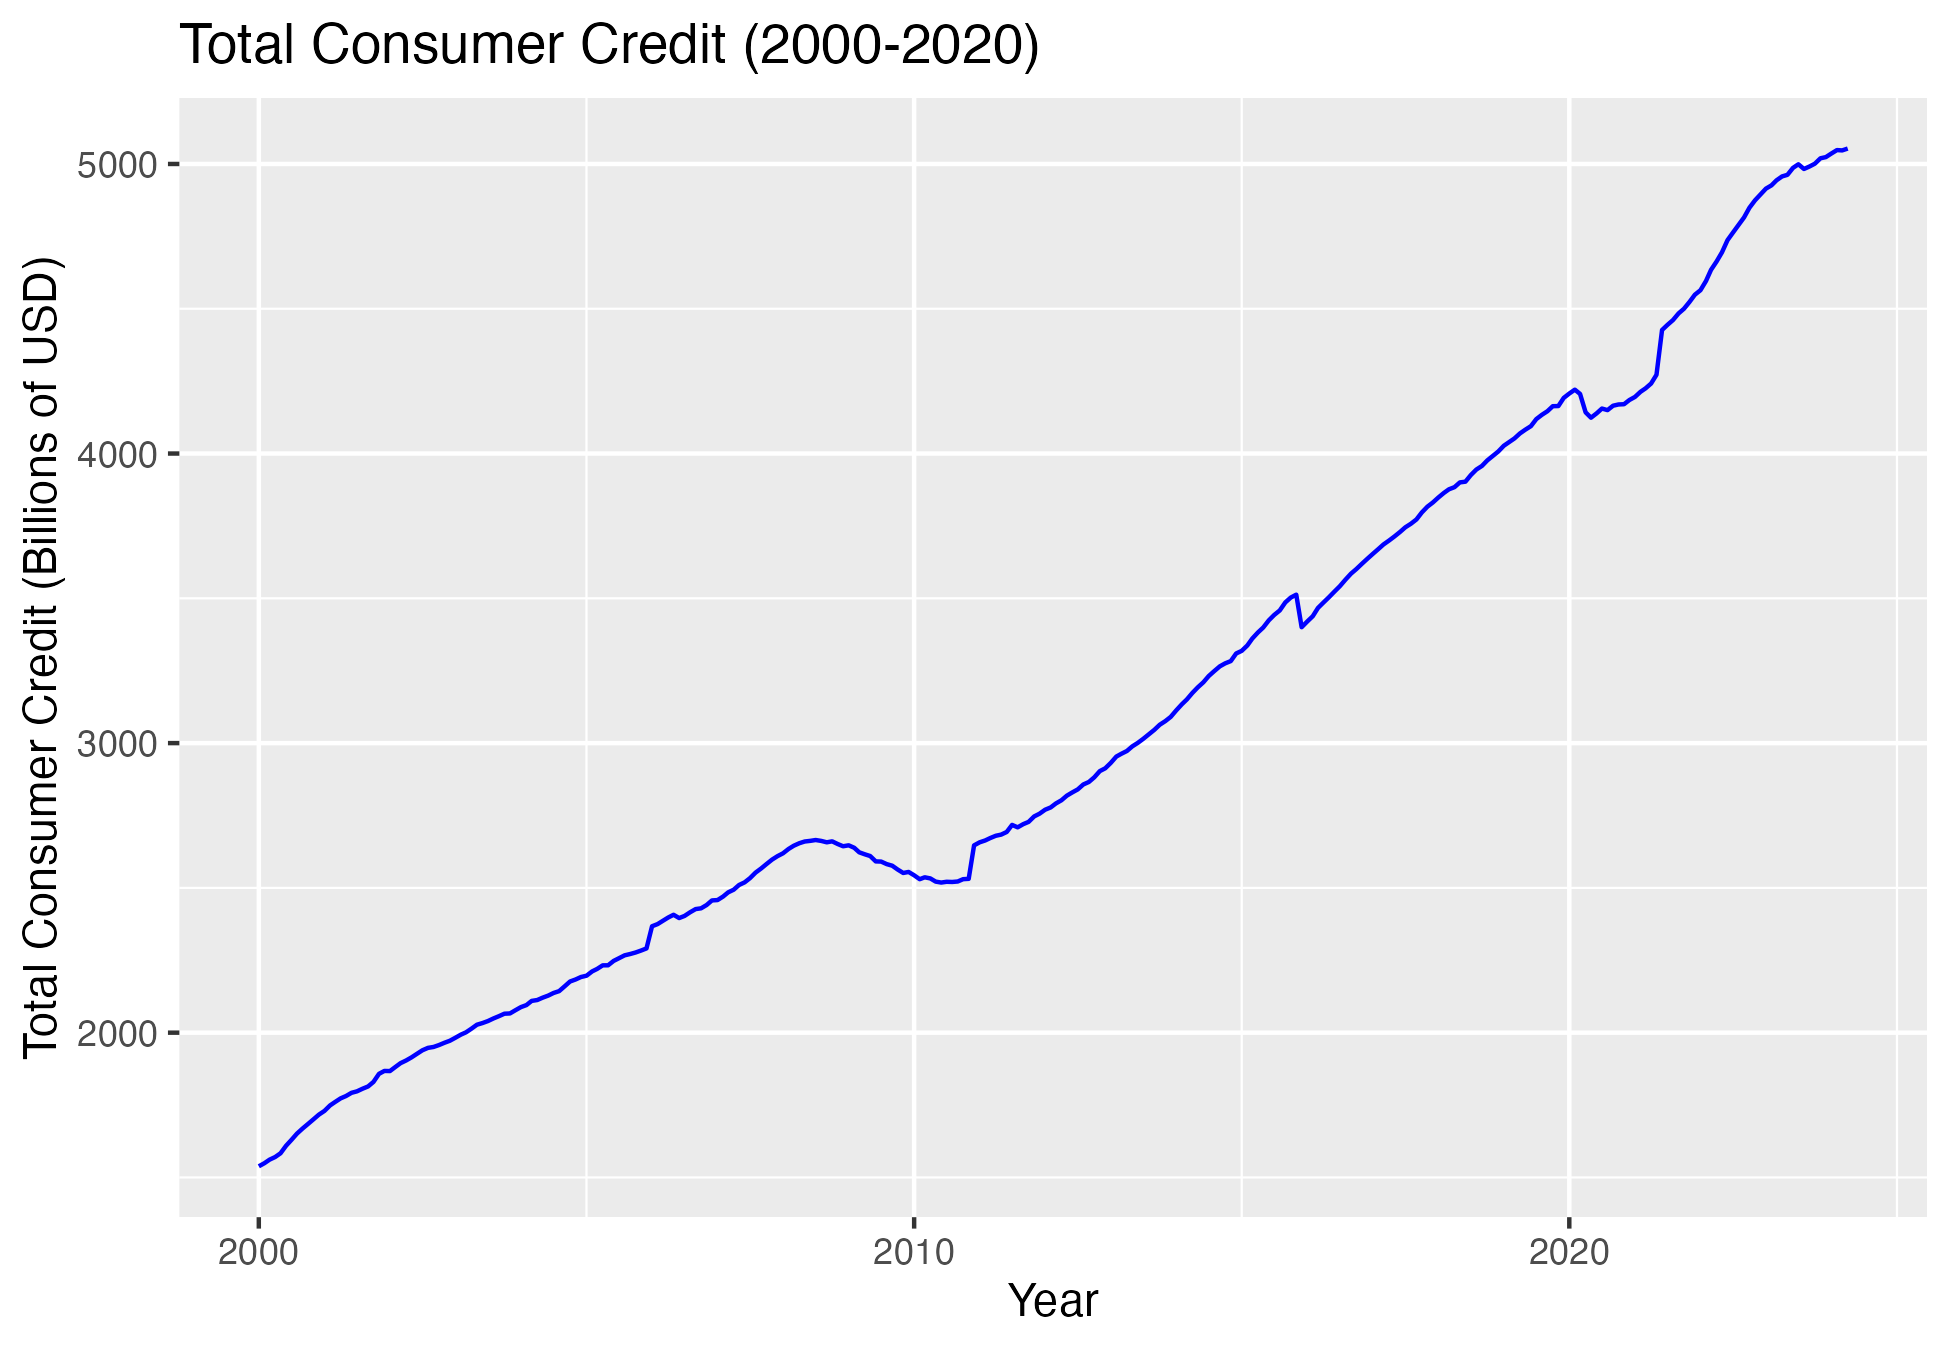
\includegraphics[width=0.9\textwidth]{/Users/cancel/Personal/Coursework/Econ425/VA1/R/Total_Consumer_Credit.png}
    \end{center}
\end{frame}

\section{Determinants of Nominal and Real Exchange Rates and the Role of UIP}
\begin{frame}
    \frametitle{Nominal and Real Exchange Rates}
    \begin{itemize}
        \item \textbf{Nominal Exchange Rate:} The rate at which one currency can be exchanged for another.
        \item \textbf{Real Exchange Rate:} Adjusts the nominal rate for differences in price levels between countries.
        \begin{gather*}
                \text{Real Exchange Rate} = \\
                \frac{\text{Nominal Exchange Rate} \times \text{Domestic Price Level}}{\text{Foreign Price Level}}
        \end{gather*}
    \end{itemize}
\end{frame}

\begin{frame}
    \frametitle{Uncovered Interest Rate Parity (UIP)}
    \begin{itemize}
        \item UIP suggests that the difference in interest rates between two countries should equal the expected change in exchange rates.
        \item Higher interest rates in one country lead to expectations of currency depreciation relative to a country with lower interest rates.
    \end{itemize}
\end{frame}

\begin{frame}
    \frametitle{Graph: Nominal Exchange Rate and Interest Rate Differential}
    \begin{center}
        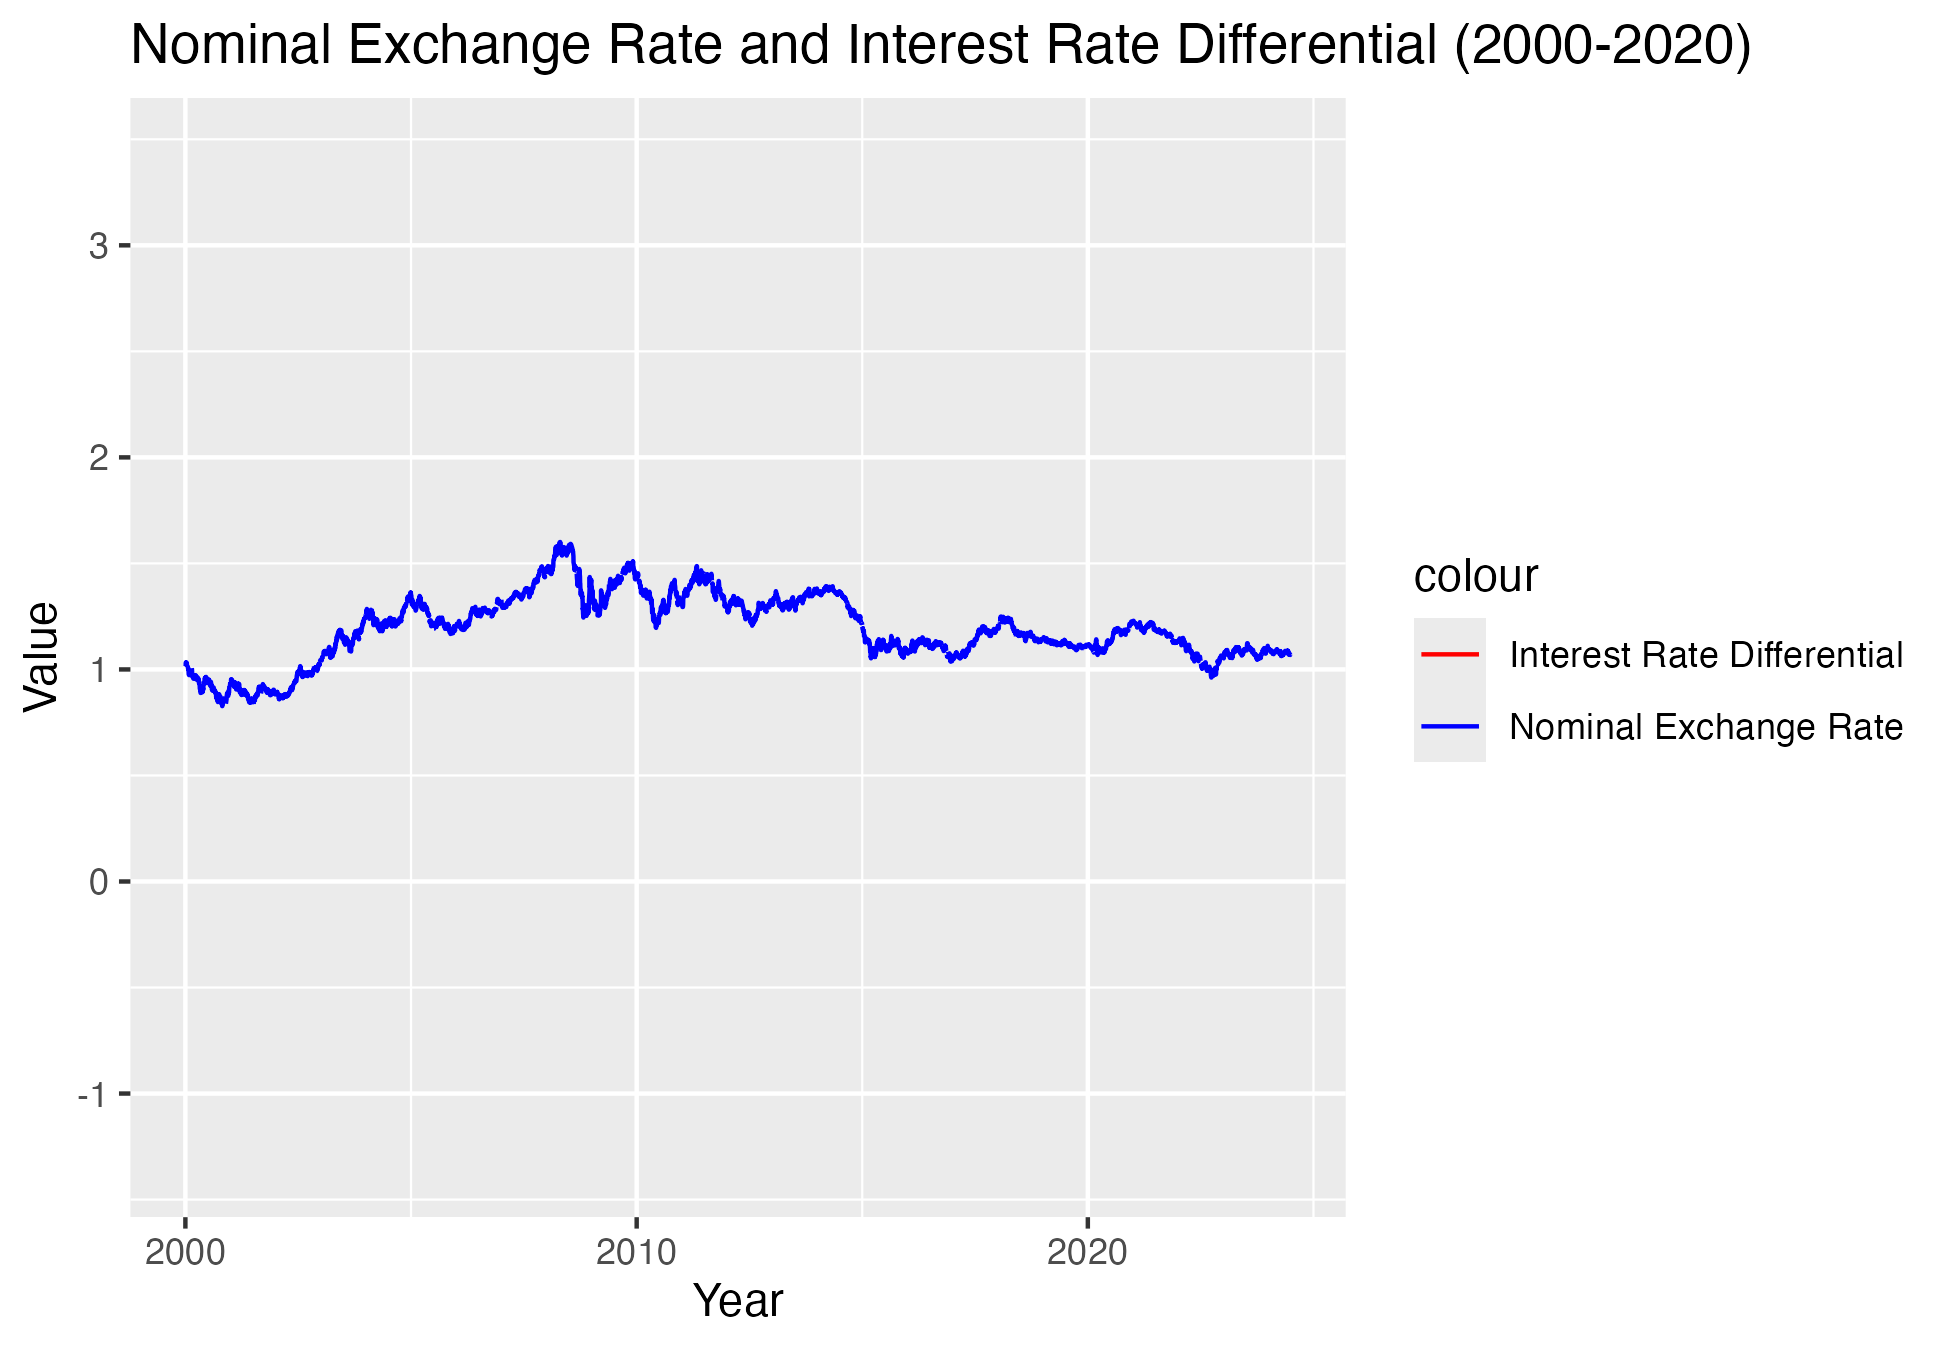
\includegraphics[width=0.9\textwidth]{/Users/cancel/Personal/Coursework/Econ425/VA1/R/Nominal_Exchange_Rate_and_Interest_Rate_Differential.png}
    \end{center}
\end{frame}

\section{Incorporating Realistic Assumptions Beyond Perfect Competition}
\begin{frame}
    \frametitle{Realistic Market Assumptions}
    \begin{itemize}
        \item \textbf{Monopolistic Competition:} Many firms sell similar but not identical products.
        \item \textbf{Oligopoly:} A few large firms dominate the market.
        \item \textbf{Market Imperfections:} Includes price stickiness, information asymmetries, and varying degrees of market power.
    \end{itemize}
\end{frame}

\section{Price Rigidity and Market Power}
\begin{frame}
    \frametitle{Price Rigidity and Market Power}
    \begin{itemize}
        \item \textbf{Price Rigidity:} Prices do not adjust immediately to changes in supply and demand.
        \item \textbf{Market Power:} Firms can set prices above marginal cost, leading to price rigidity.
        \item \textbf{Macroeconomic Implications:} Prolonged disequilibrium, unemployment, or shortages, and slower response to economic shocks.
    \end{itemize}
\end{frame}

\begin{frame}
    \frametitle{Graph: Consumer Price Index}
    \begin{center}
        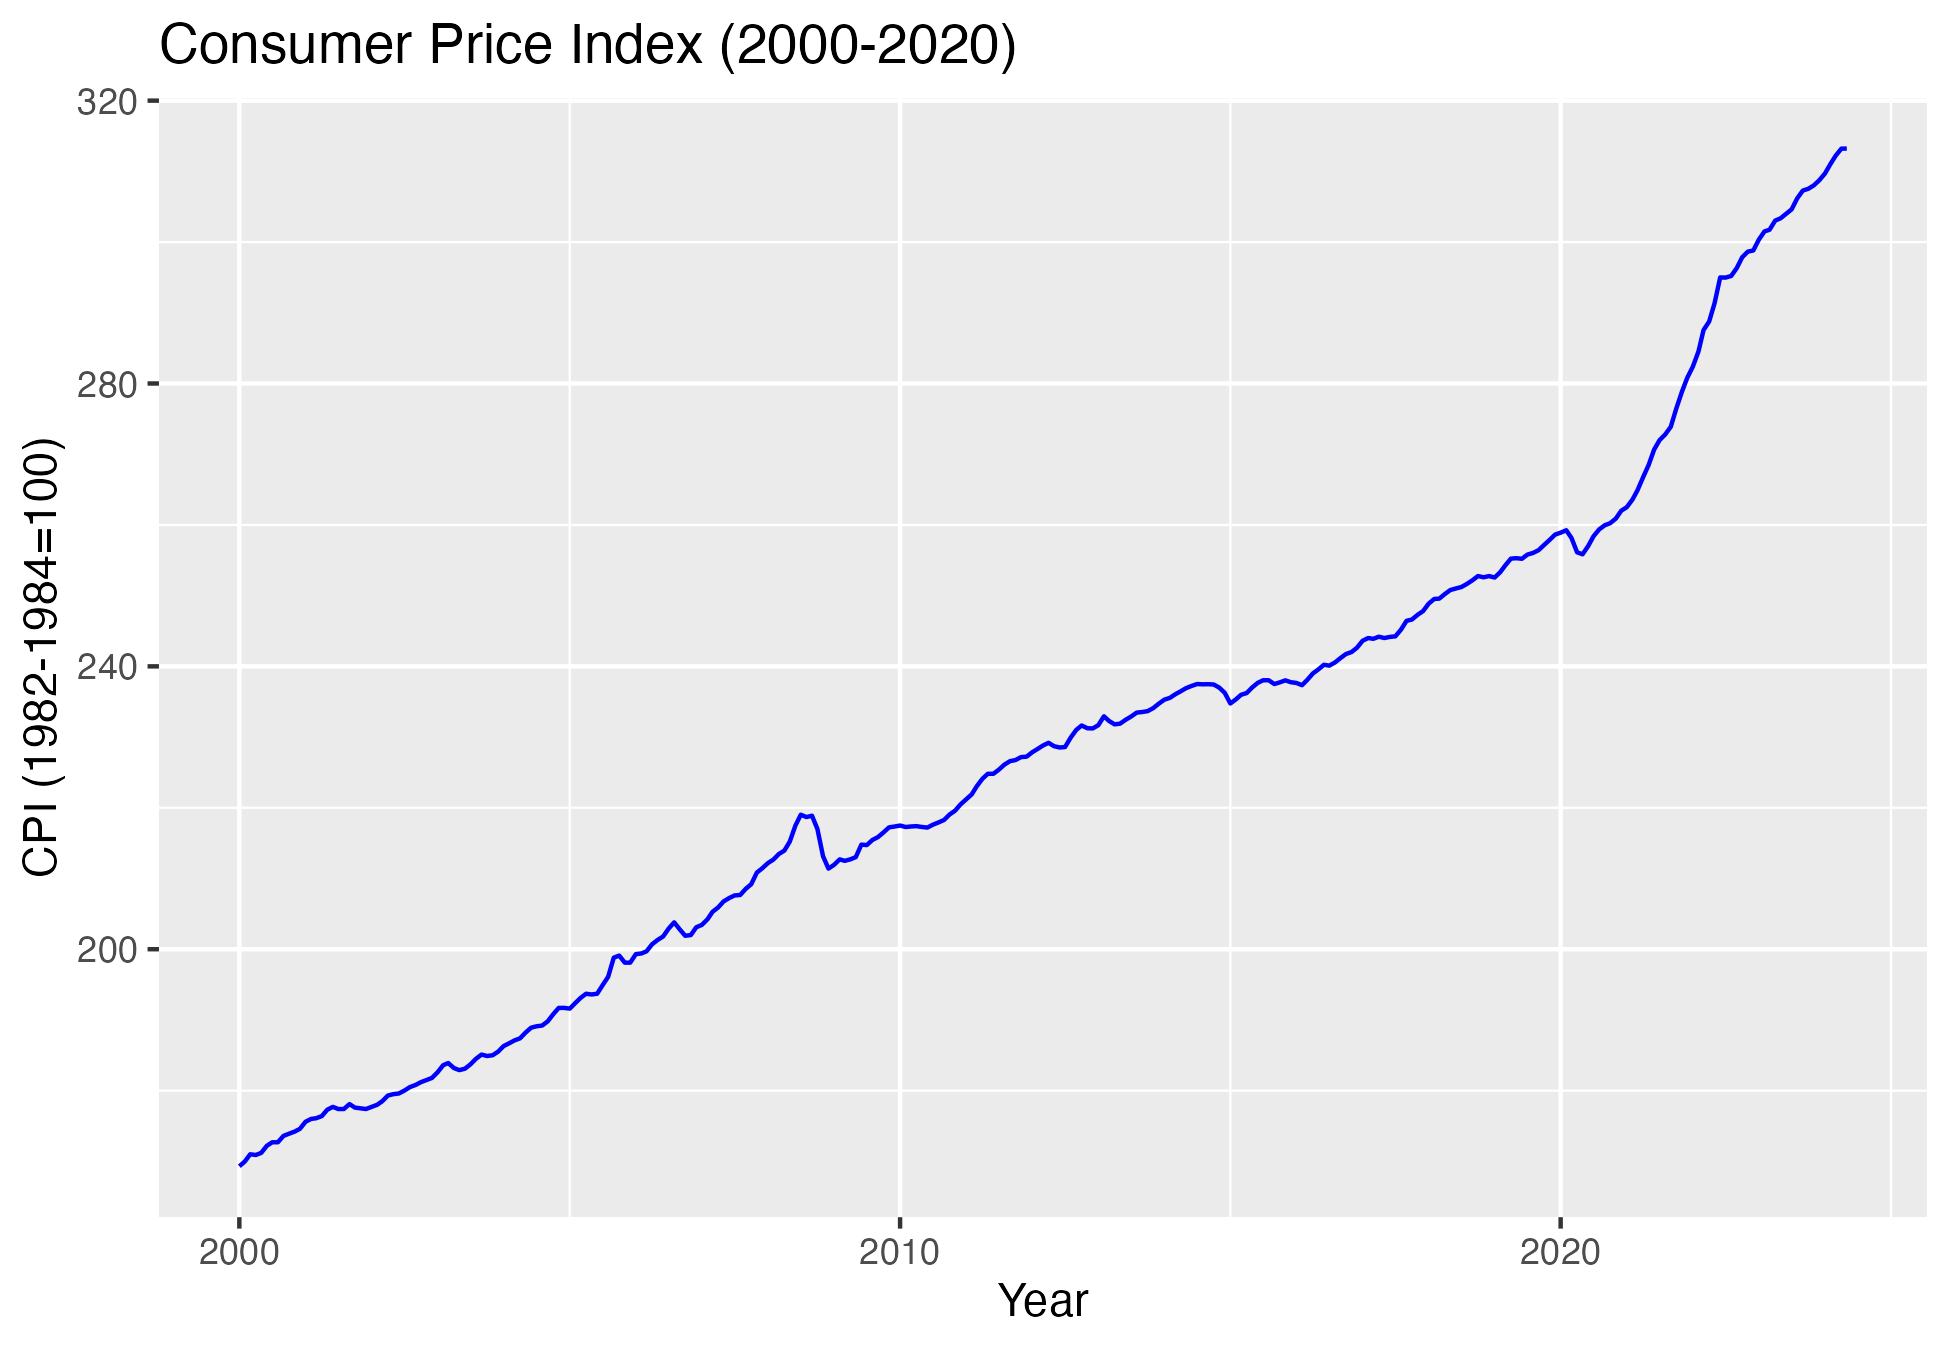
\includegraphics[width=0.9\textwidth]{/Users/cancel/Personal/Coursework/Econ425/VA1/R/Consumer_Price_Index.png}
    \end{center}
\end{frame}

\section{Natural Level of Output and Output Gap}
\begin{frame}
    \frametitle{Natural Level of Output and Output Gap}
    \begin{itemize}
        \item \textbf{Natural Level of Output:} The level of production when the economy operates at full capacity.
        \item \textbf{Output Gap:} The difference between actual output and potential output.
        \begin{itemize}
            \item Positive Output Gap: Actual output exceeds potential output.
            \item Negative Output Gap: Actual output is below potential output.
        \end{itemize}
        \item \textbf{Natural Rate Hypothesis:} The economy tends towards the natural rate of unemployment and output in the long run.
    \end{itemize}
\end{frame}

\begin{frame}
    \frametitle{Graph: Actual vs. Potential Output}
    \begin{center}
        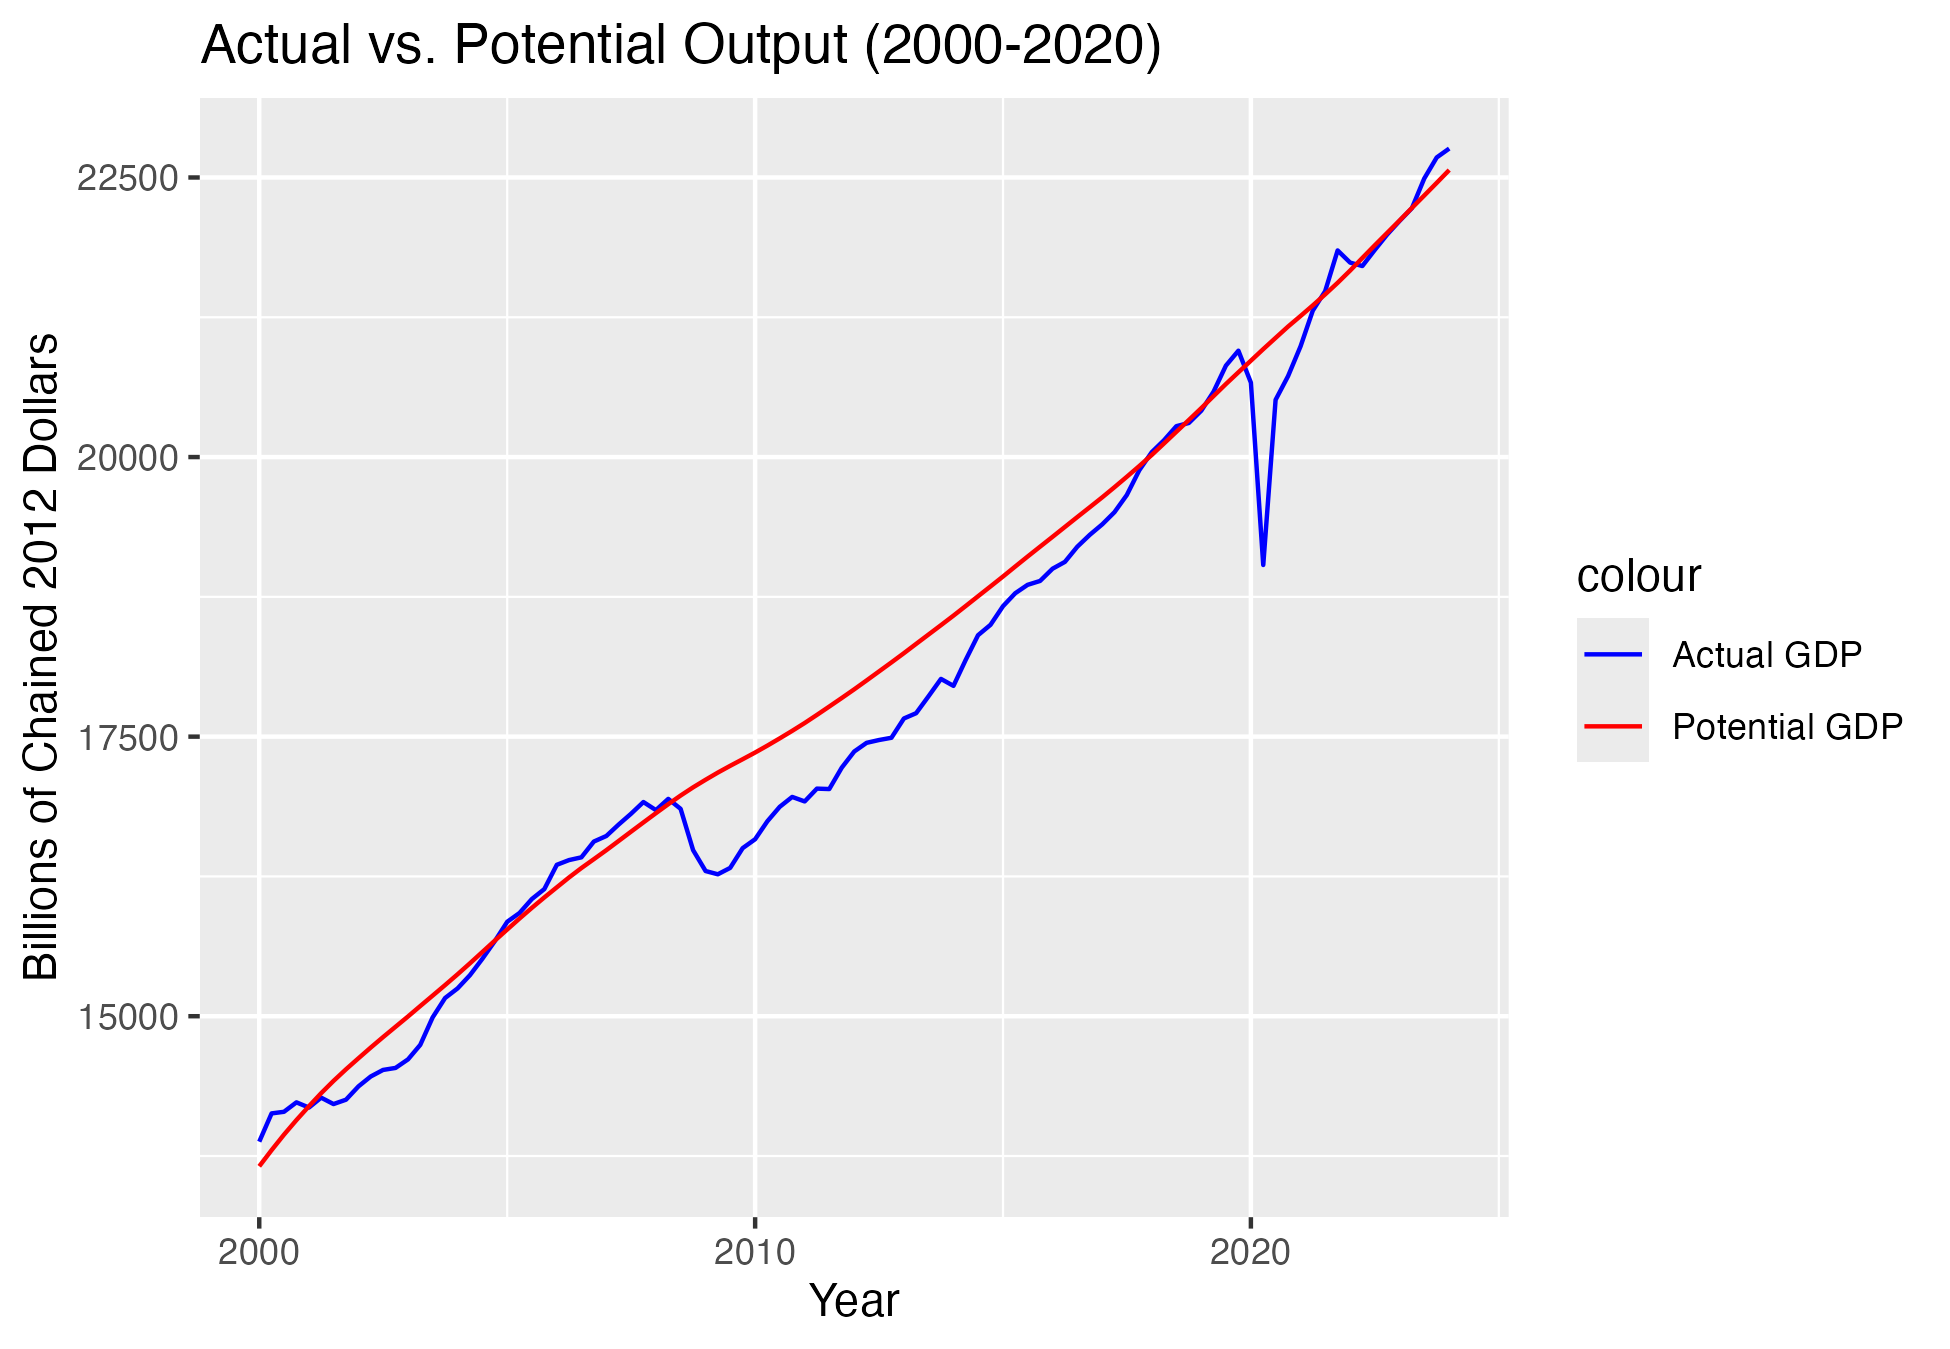
\includegraphics[width=0.9\textwidth]{/Users/cancel/Personal/Coursework/Econ425/VA1/R/Actual_vs_Potential_Output.png}
    \end{center}
\end{frame}

\section{Phillips Curve}
\begin{frame}
    \frametitle{Phillips Curve}
    \begin{itemize}
        \item \textbf{Phillips Curve:} Represents the inverse relationship between inflation and unemployment in the short run.
        \item Named after economist A.W. Phillips.
    \end{itemize}
\end{frame}

\begin{frame}
    \frametitle{Graph: Phillips Curve}
    \begin{center}
        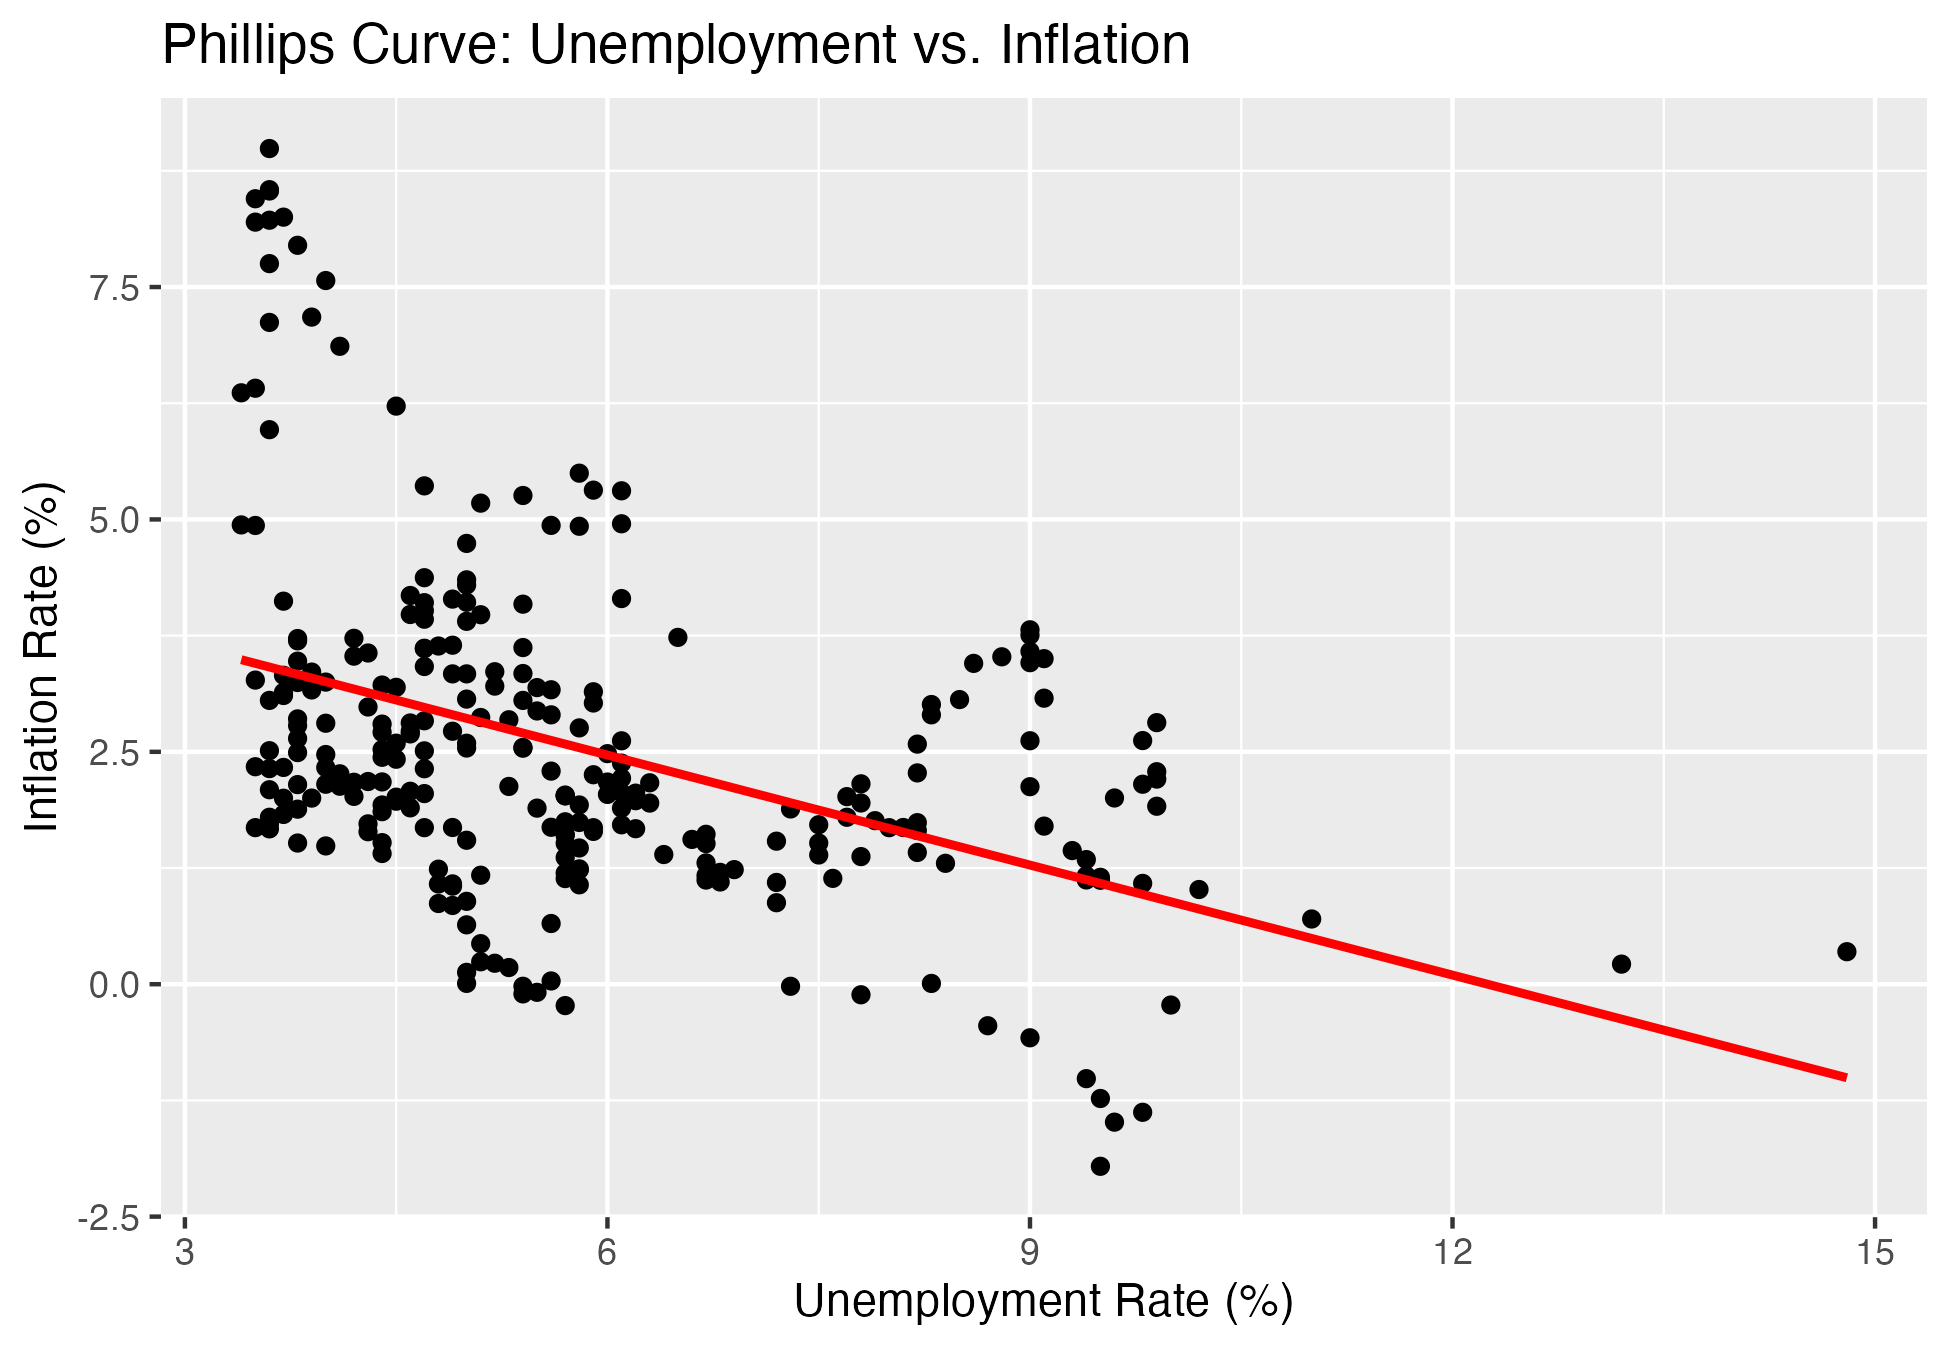
\includegraphics[width=0.9\textwidth]{/Users/cancel/Personal/Coursework/Econ425/VA1/R/Phillips_Curve.png}
    \end{center}
\end{frame}

\section{Shocks in Macroeconomics}
\begin{frame}
    \frametitle{Shocks in Macroeconomics}
    \begin{itemize}
        \item \textbf{Shock:} An unexpected event affecting the economy.
        \item \textbf{Types of Shocks:}
        \begin{itemize}
            \item Supply Shock: Affects the supply side (e.g., oil price increase).
            \item Demand Shock: Affects the demand side (e.g., increase in consumer confidence).
        \end{itemize}
    \end{itemize}
\end{frame}

\begin{frame}
    \frametitle{Graph: Impact of Supply Shocks on GDP}
    \begin{center}
        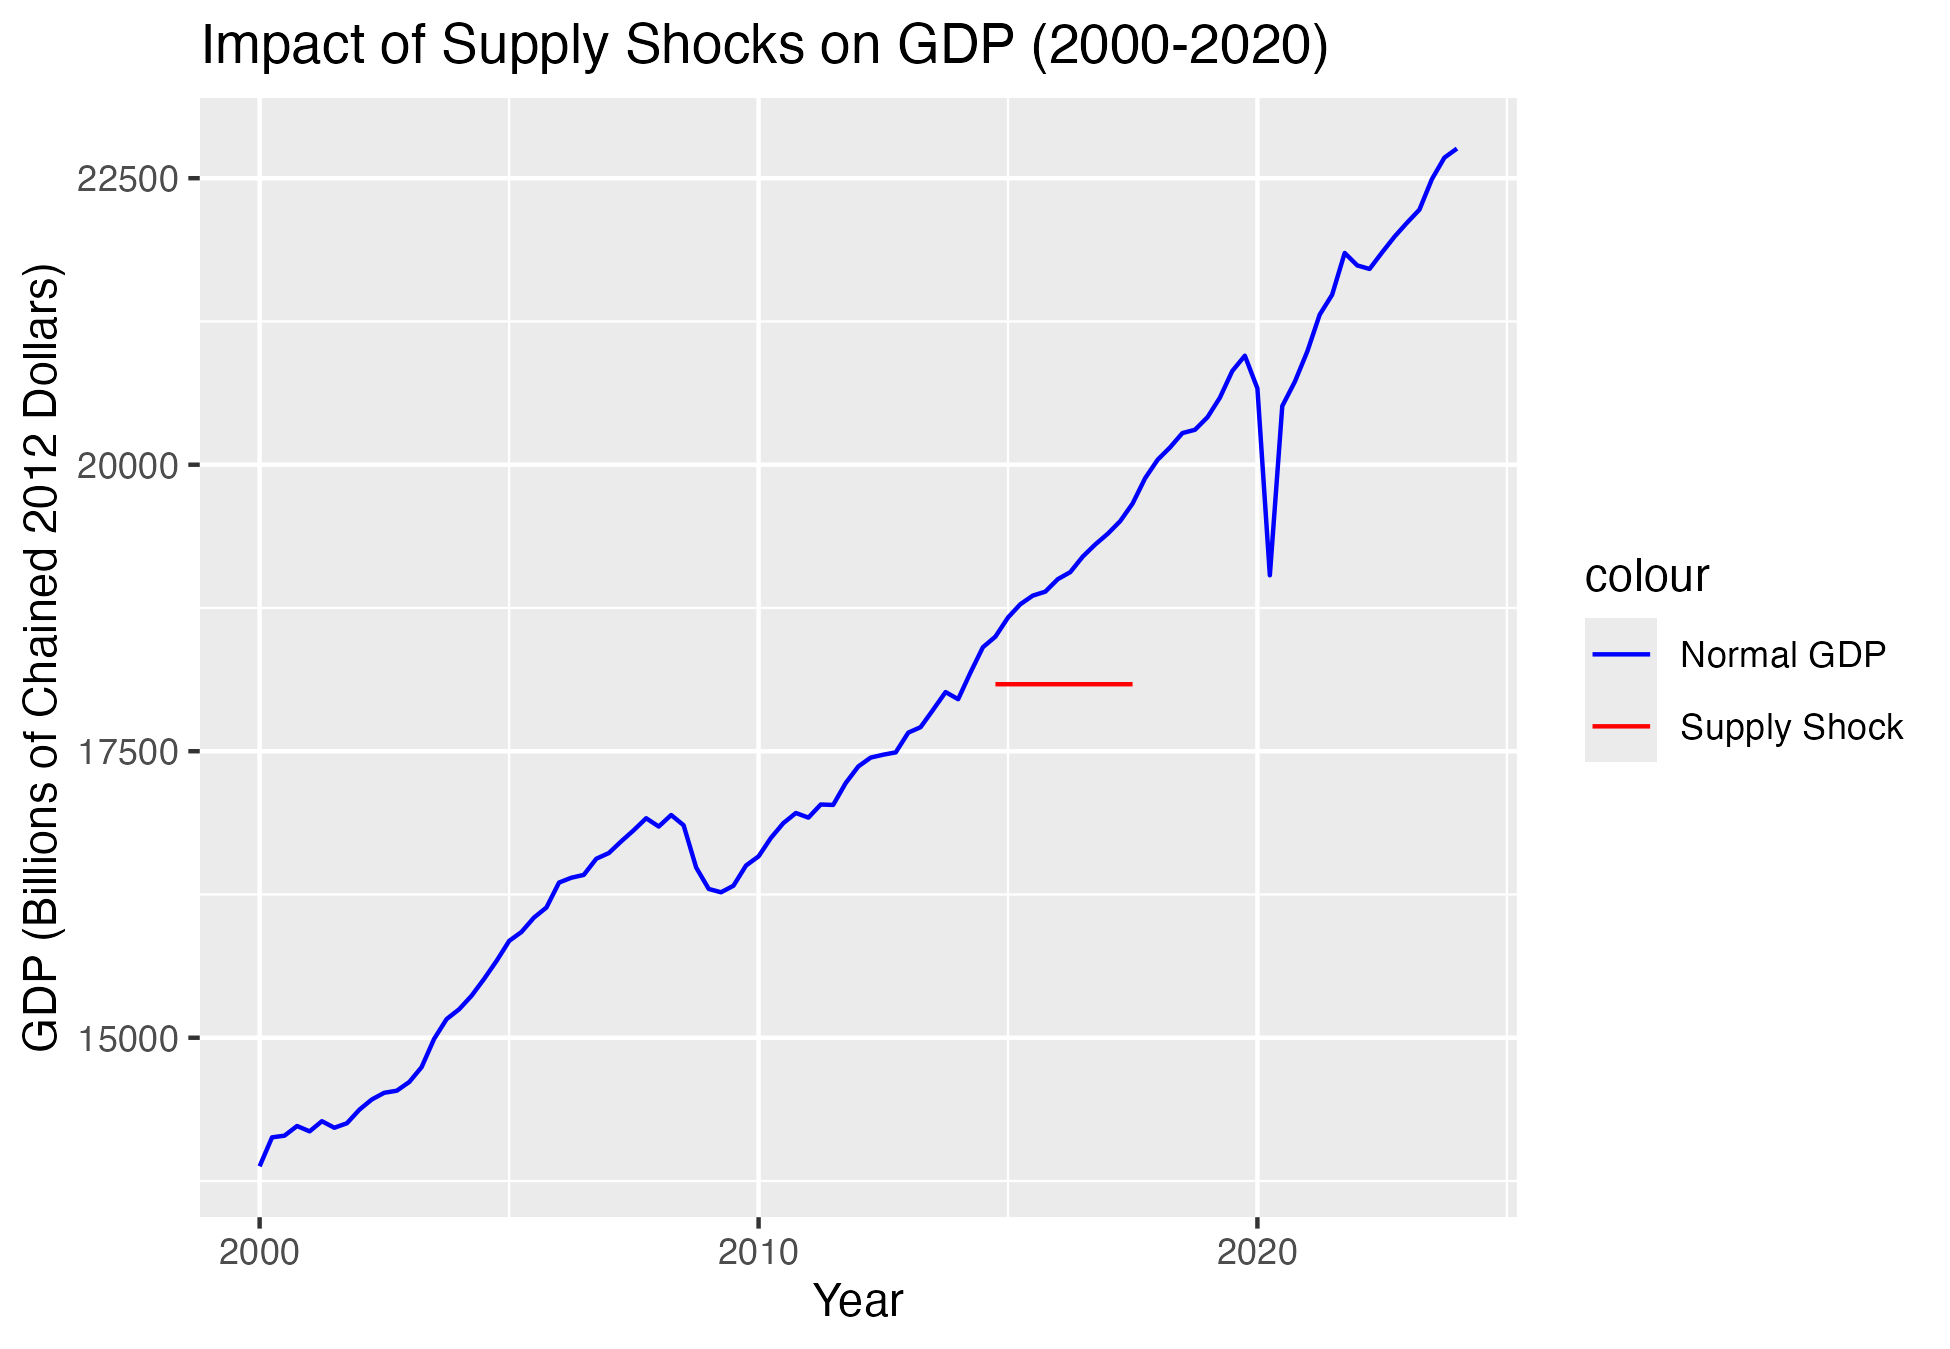
\includegraphics[width=0.9\textwidth]{/Users/cancel/Personal/Coursework/Econ425/VA1/R/Impact_of_Supply_Shocks_on_GDP.png}
    \end{center}
\end{frame}

\section{Monetary Policy Shock as an AD Shock}
\begin{frame}
    \frametitle{Monetary Policy Shock as an AD Shock}
    \begin{itemize}
        \item \textbf{Monetary Policy Shock:} An unexpected change in monetary policy.
        \item \textbf{Aggregate Demand (AD) Shock:}
        \begin{itemize}
            \item Expansionary Policy: Lower interest rates or increased money supply boost consumption and investment.
            \item Contractionary Policy: Higher interest rates or reduced money supply reduce consumption and investment.
        \end{itemize}
    \end{itemize}
\end{frame}

\begin{frame}
    \frametitle{Graph: Impact of Monetary Policy on GDP}
    \begin{center}
        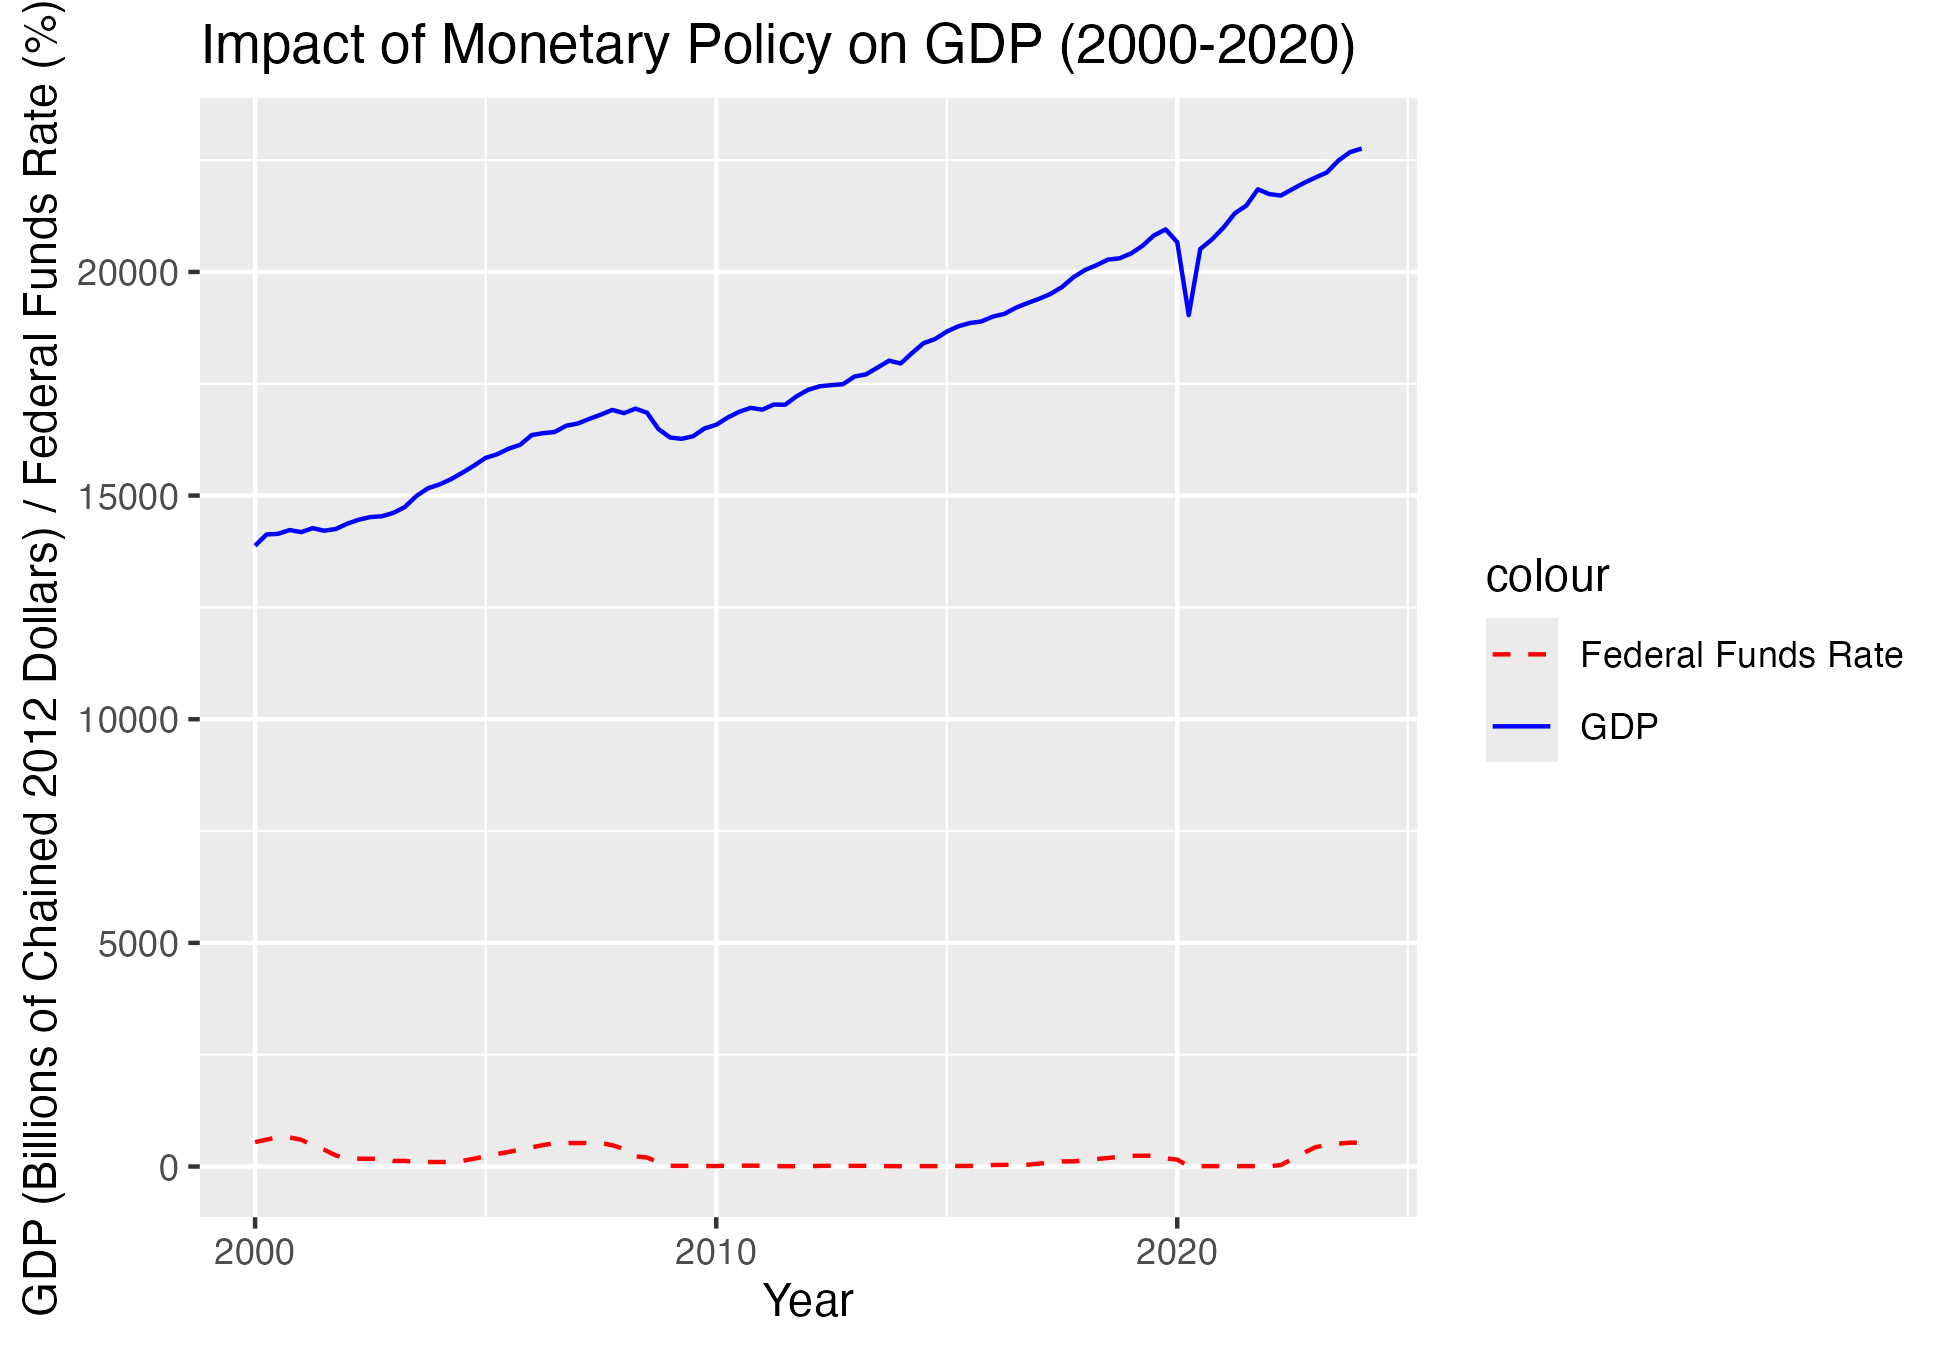
\includegraphics[width=0.9\textwidth]{/Users/cancel/Personal/Coursework/Econ425/VA1/R/Impact_of_Monetary_Policy_on_GDP.png}
    \end{center}
\end{frame}

\section{Productivity Shock Mechanism}
\begin{frame}
    \frametitle{Productivity Shock Mechanism}
    \begin{itemize}
        \item \textbf{Productivity Shock:} A sudden change in the productivity of labor or capital.
        \item \textbf{Mechanism:}
        \begin{itemize}
            \item Positive Productivity Shock: Increases output, lowers prices, and can lead to higher wages and employment.
            \item Negative Productivity Shock: Reduces output, raises prices, and can lead to lower wages and employment.
        \end{itemize}
    \end{itemize}
\end{frame}

\begin{frame}
    \frametitle{Graph: Impact of Productivity Shocks on GDP}
    \begin{center}
        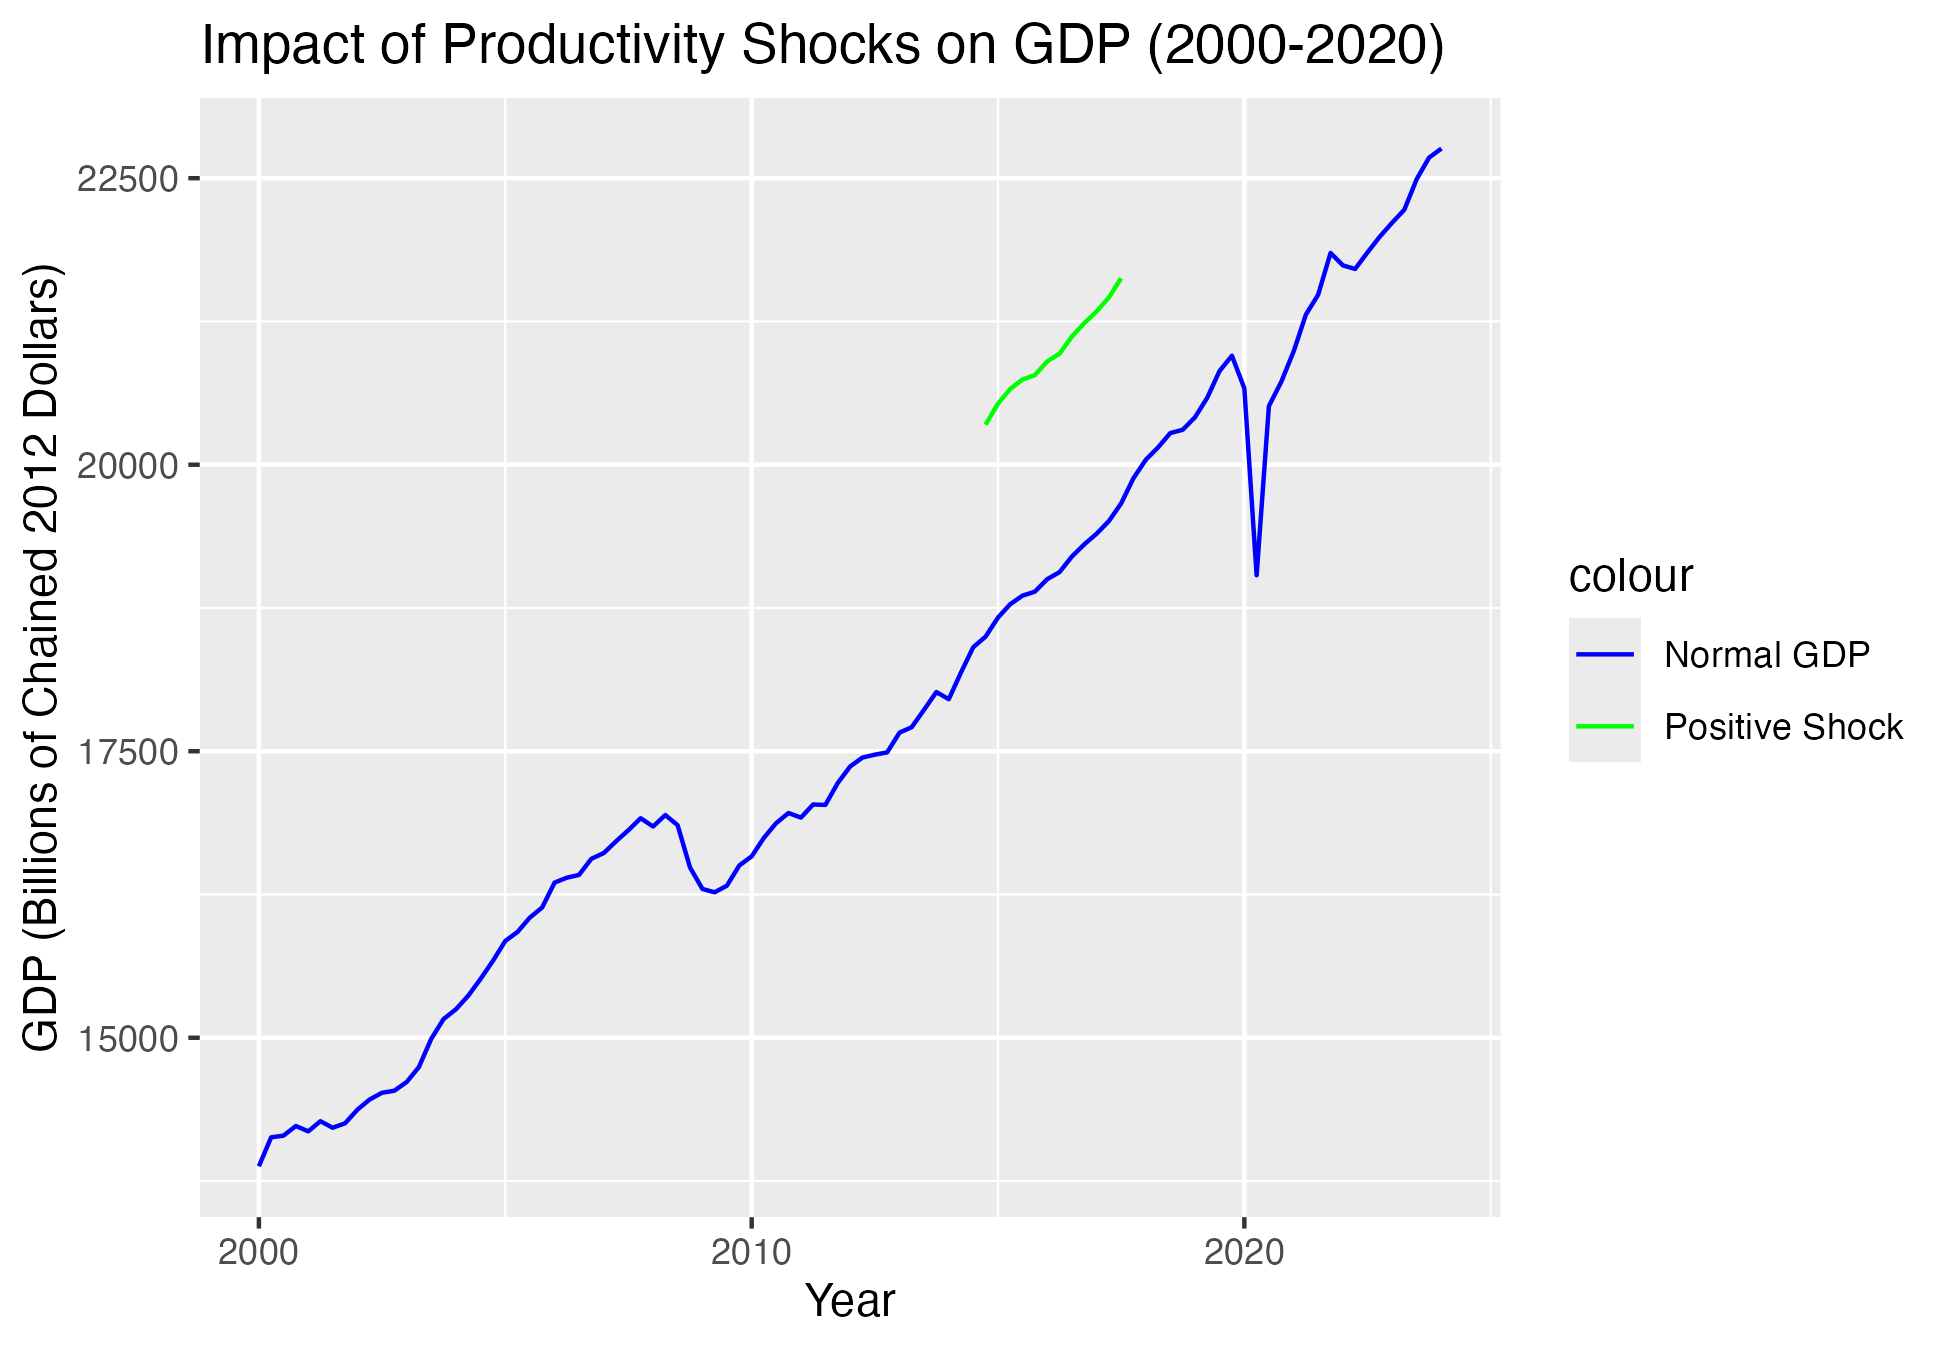
\includegraphics[width=0.9\textwidth]{/Users/cancel/Personal/Coursework/Econ425/VA1/R/Impact_of_Productivity_Shocks_on_GDP.png}
    \end{center}
\end{frame}

\section{Business Cycles}
\begin{frame}
    \frametitle{Business Cycles}
    \begin{itemize}
        \item \textbf{Business Cycles:} Fluctuations in economic activity characterized by periods of expansion and contraction.
        \begin{itemize}
            \item Expansion: Increasing economic activity, rising GDP, and falling unemployment.
            \item Peak: The highest point of economic activity before a downturn.
            \item Contraction: Decreasing economic activity, falling GDP, and rising unemployment.
            \item Trough: The lowest point of economic activity before a recovery begins.
        \end{itemize}
        \item \textbf{Importance for Macroeconomic Policy:} Policymakers aim to smooth out these cycles to achieve stable economic growth, low unemployment, and stable inflation.
    \end{itemize}
\end{frame}

\begin{frame}
    \frametitle{Graph: Business Cycles}
    \begin{center}
        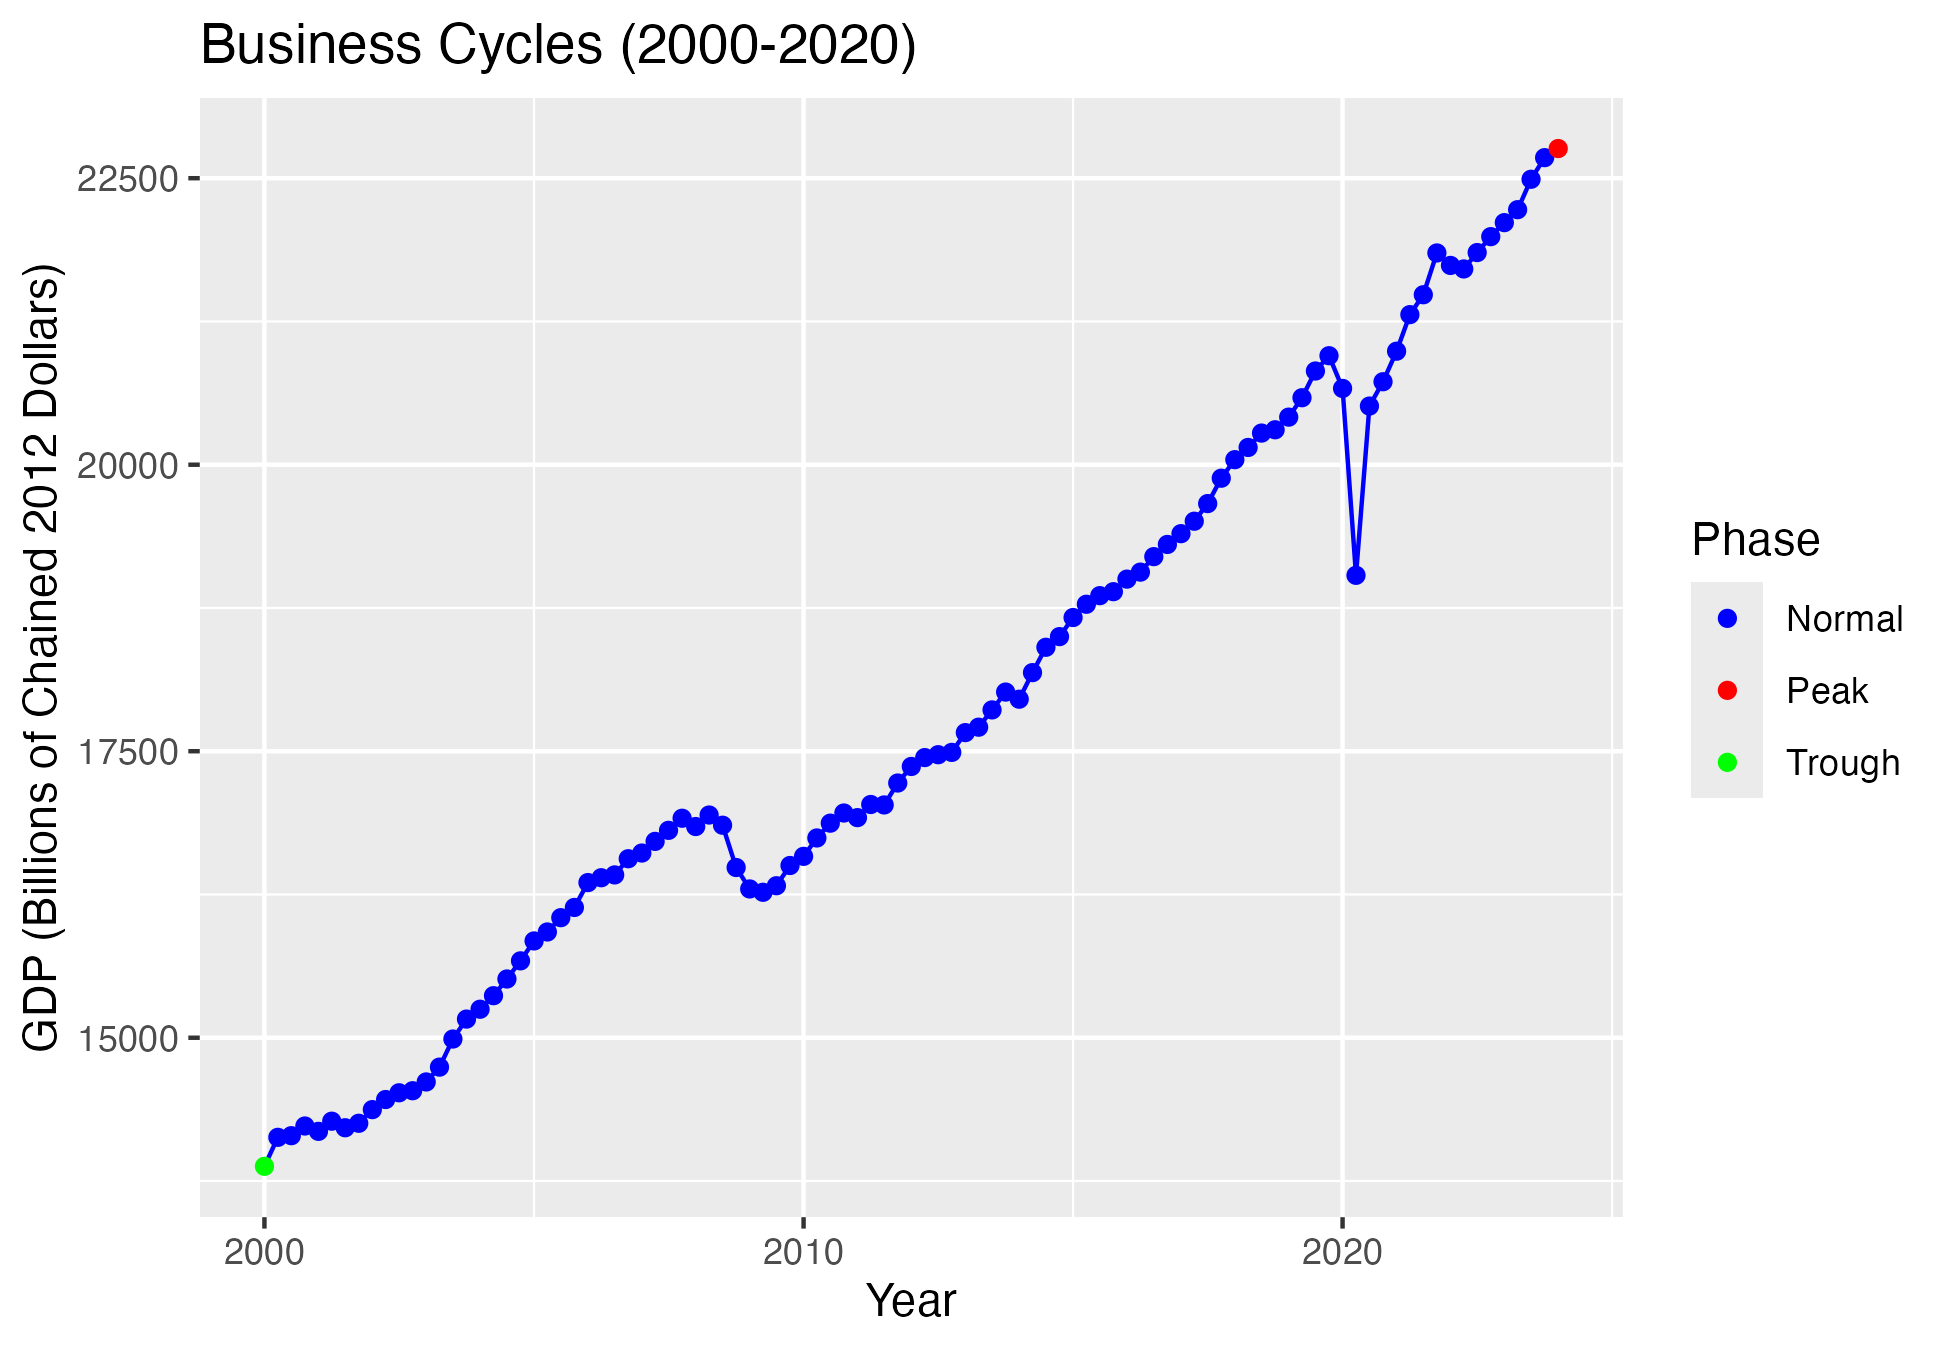
\includegraphics[width=0.9\textwidth]{/Users/cancel/Personal/Coursework/Econ425/VA1/R/Business_Cycles.png}
    \end{center}
\end{frame}

\section{HP Filter and Cyclical Variables}
\begin{frame}
    \frametitle{HP Filter and Cyclical Variables}
    \begin{itemize}
        \item \textbf{HP Filter:} A statistical tool used to separate the cyclical component of a time series from its trend component.
        \item \textbf{Procyclical vs. Countercyclical Variables:}
        \begin{itemize}
            \item Procyclical Variable: Moves in the same direction as the overall economy (e.g., investment, consumer spending).
            \item Countercyclical Variable: Moves in the opposite direction to the overall economy (e.g., unemployment, government spending on social programs).
        \end{itemize}
    \end{itemize}
\end{frame}

\begin{frame}
    \frametitle{Graph: HP Filter Applied to GDP}
    \begin{center}
        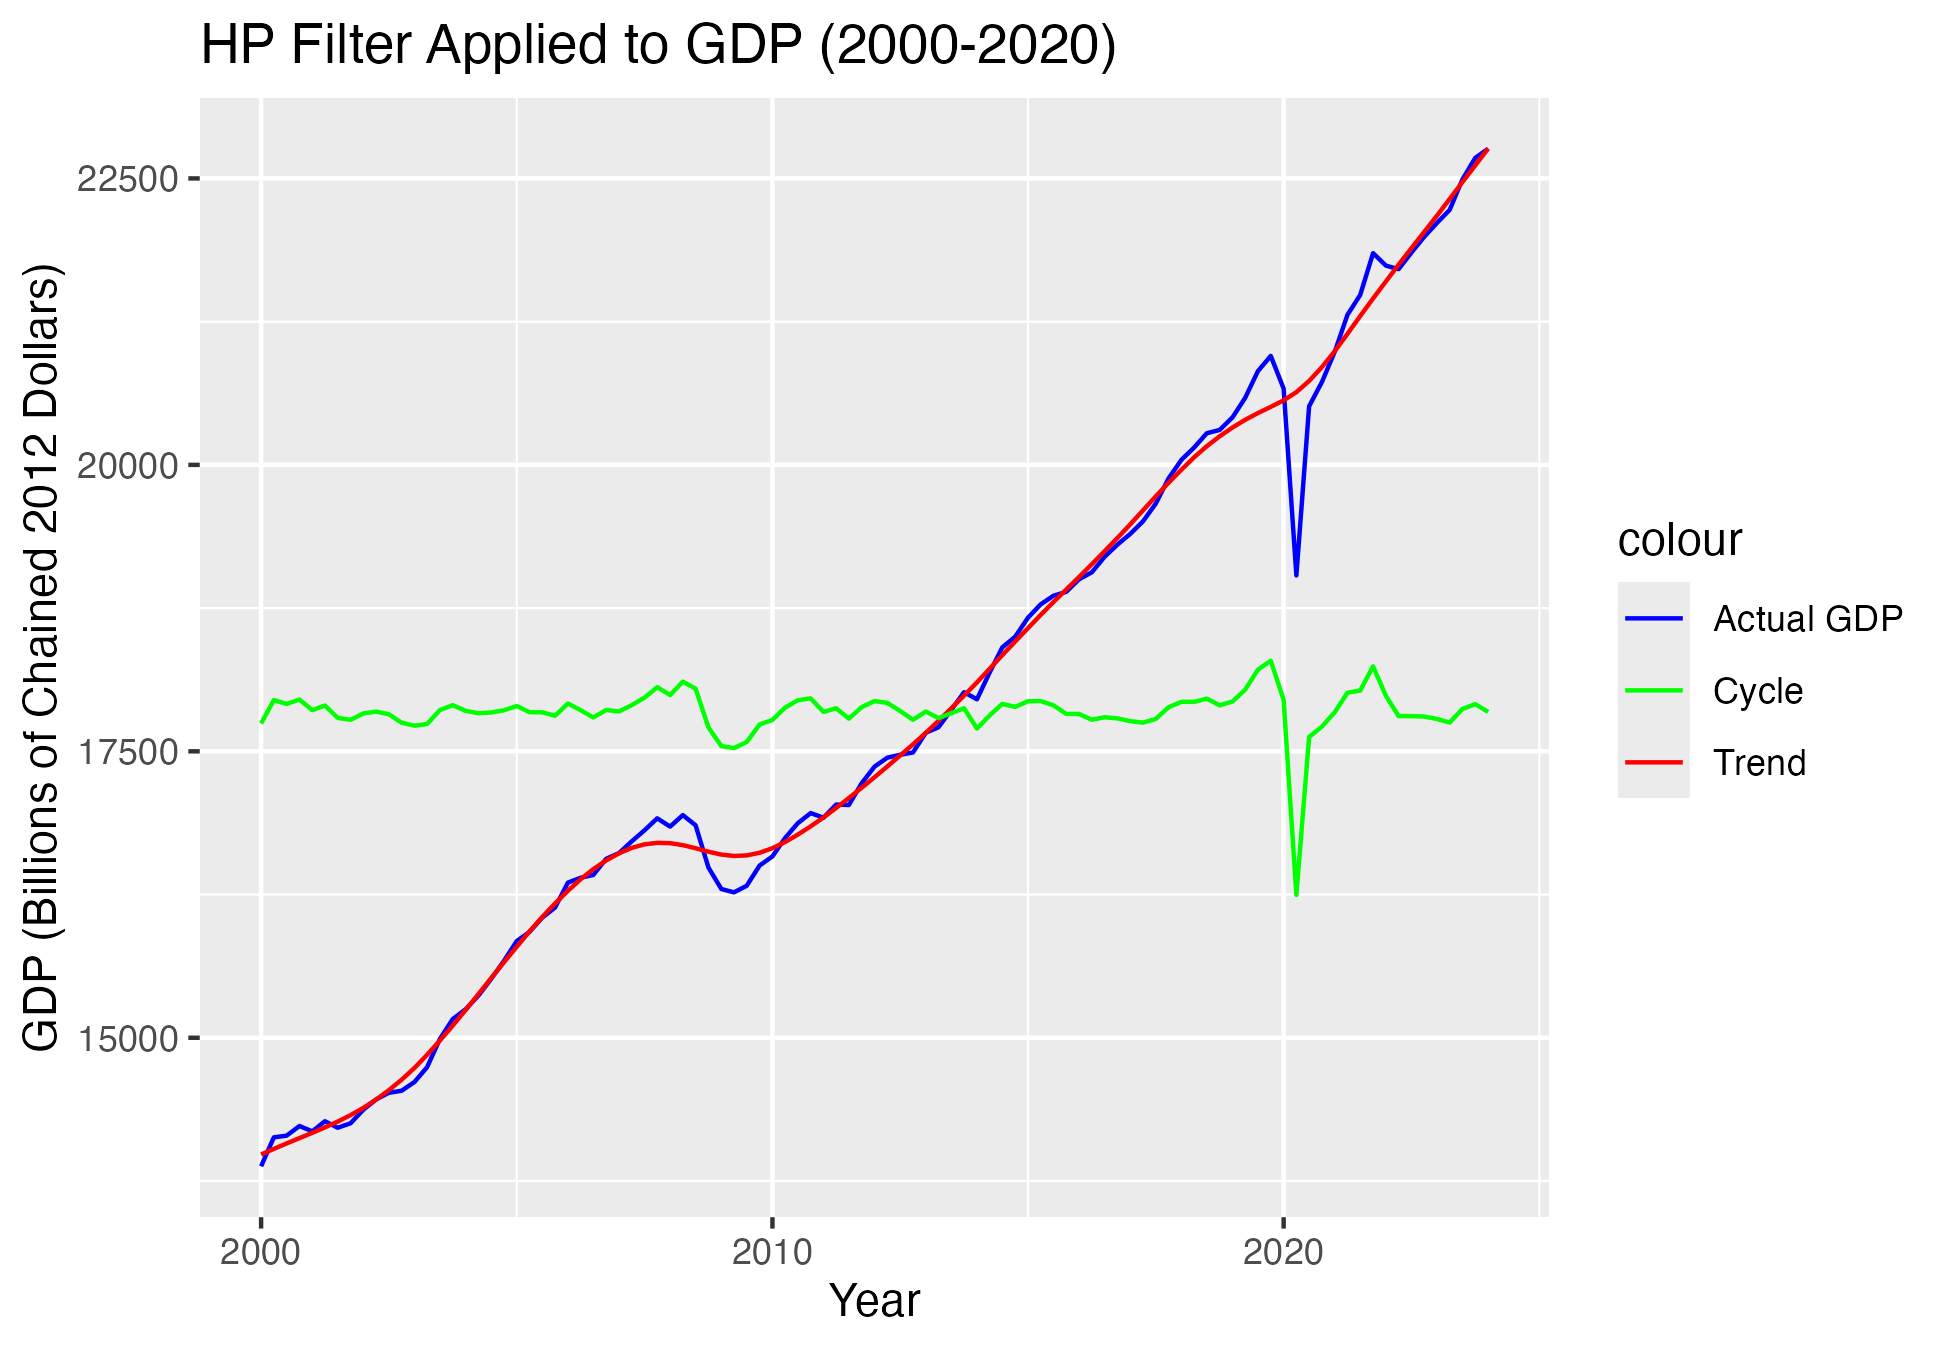
\includegraphics[width=0.9\textwidth]{/Users/cancel/Personal/Coursework/Econ425/VA1/R/HP_Filter_Applied_to_GDP.png}
    \end{center}
\end{frame}

\end{document}
